\documentclass[tcc]{subfiles}

\begin{document}

\chapter{Dynamic engine model}
\label{ch:engine_model}
\epigraph{\em ``It's not denial.\\ I'm just selective about the reality I
accept.''}{\em(Bill Watterson)}

To develop a controller for any kind of system,
 the first thing needed is a model which reproduces the system's behavior in time.
 i.e.\ a dynamic or transient model.
 For the present work, we must model a gas turbine engine.

The engine model used is of the lumped volume type. This means that each component 
 (compressor, combustor,turbine and nozzle)
 is modelled as a single point in space and conservation laws are applied to them.
 This type of model is also known as zero dimensional (0-D) or as parametric cycle analysis
 \index{parametric cycle analysis},
 and is widely used in both industry and academy as a tool for preliminary design and 
 performance analysis. 

There are many readily available computer programs that implement this kind of simulation. 
From these, the most famous is probably the commercial program GasTurb \cite{GasTurb}, 
\index{software} \index{GasTurb}
followed by the \gls{GSP} \cite{Visser2000}.
A comparison of both is presented in \textcite{GasTurbvsGSP}.
In particular, GasTurb has already been used to simulate model gas turbines 
 \cite{gao2011modelling}.
An open-source alternative is the \gls{T-MATS}, from NASA \cite{T-MATS}.
\gls{T-MATS} provides a library of turbo machinery blocks for use in Simulink. 
Each of these blocks is actually a wrapper for a function written in C 
 that simulates the component's behaviour.

A schematic of the engine components considered for the simulation of the present gas turbine engine is shown in \todo{add figure}.

\section{Model description}

The thermodynamic model of a gas turbine is described in terms of dimensionless parameters.%
\index{parameters!dimensionless}
These are parameters obtained by the Buckingham $\pi$ theorem, 
 and they greatly reduce the number of variables involved in the performance analysis.
 They are able to implicitly account for variations in ambient pressure and temperature, 
 gas properties and engine dimensions, for example.
If we fix the working fluid and the engine dimensions, the terms related to gas properties and areas can be dropped from the dimensionless parameters and we obtain the quasi-dimensionless parameters.
\index{parameters!quasi-dimensionless}
The quasi-dimensionless parameters account implicitly for variations in ambient pressure and temperature only.
They are dimensional terms, but do not have a clear physical interpretation. 
To make engineering judgement easier, it is useful to scale these parameters by 
 a standard pressure and temperature, which are usually taken as the 
 \gls{ISA} conditions at \gls{SL}. 
In this manner, they are a function of the terms theta (\acs{theta}) and delta (\acs{delta}):
\begin{align}
    \acs{delta} &= \text{inlet pressure}/\text{\acs{ISA} pressure at \acs{SL}} \\
    \acs{theta} &= \text{inlet temperature}/\text{\acs{ISA} temperature at \acs{SL}}
\end{align}
The parameters obtained in this way are called \emph{corrected} or \emph{referred}.
\index{parameters!corrected}
\index{parameters!referred| see {parameters, corrected}}
They retain the dimension of the physical quantity they represent, 
 and can be thought as to represent the engine performance at standard sea level conditions.
\cite{walsh2004gas}. 
The \emph{corrected parameters} will be used for the engine model,
 and are described in table \todo{add table}.

 %%Provisional table, this will be removed.
 \includepdf[pages=166-169]{references/walsh2004gas-Gas_Turbine_Performance.pdf}

 
The turbo machinery components of the engine are characterized using component maps.%
\index{component map}
 These are plots that relate corrected shaft rotation speed, corrected temperature,
 corrected mass flow and isentropic efficiency for the turbine and compressor.
Typical component maps are shown in \todo{add figures}

Seen in the framework of control theory,
 a single shaft turbine is a system with one state and two inputs.
 The inputs are corrected fuel flow and flight mach number 
 and the state is the corrected shaft rotational speed.
 Every other corrected engine parameter, such as shaft acceleration and thrust,
 can be derived from this two by an off-design calculation
 which allows for excess power in the turbine.
This calculation is the thermodynamic model of the engine and is highly non-linear and depends on the knowledge of the behaviour of each of the engine component.

The calculation process works as follows.
Inlet mach number, corrected shaft rotational speed and corrected fuel flow are known.
A value for the corrected mass flow is guessed and with the compressor map the compressor pressure ratio in obtained, along with its efficiency.
This allow the corrected pressure and temperature downstream of the compressor to be obtained.
The fuel flow allows the increase in enthalpy in the combustion chamber to be calculated, and thus the conditions at the turbine inlet.
The turbine map is then used to obtain the conditions downstream of the turbine, and the propulsive nozzle is calculated using quasi-unidimensional compressible flow theory \cite{anderson}.
The calculation of the propulsive nozzle provides a new value for the corrected mass flow, which is used to update the initial guess until 
 convergence is achieved.
This process is shown as a flowchart in \cref{fig:transient_calculation}.

\todo{Figure: transient calculation flowchart}
\begin{figure}
    \centering
    \caption{Transient calculation flowchart}
    \label{fig:transient_calculation}
    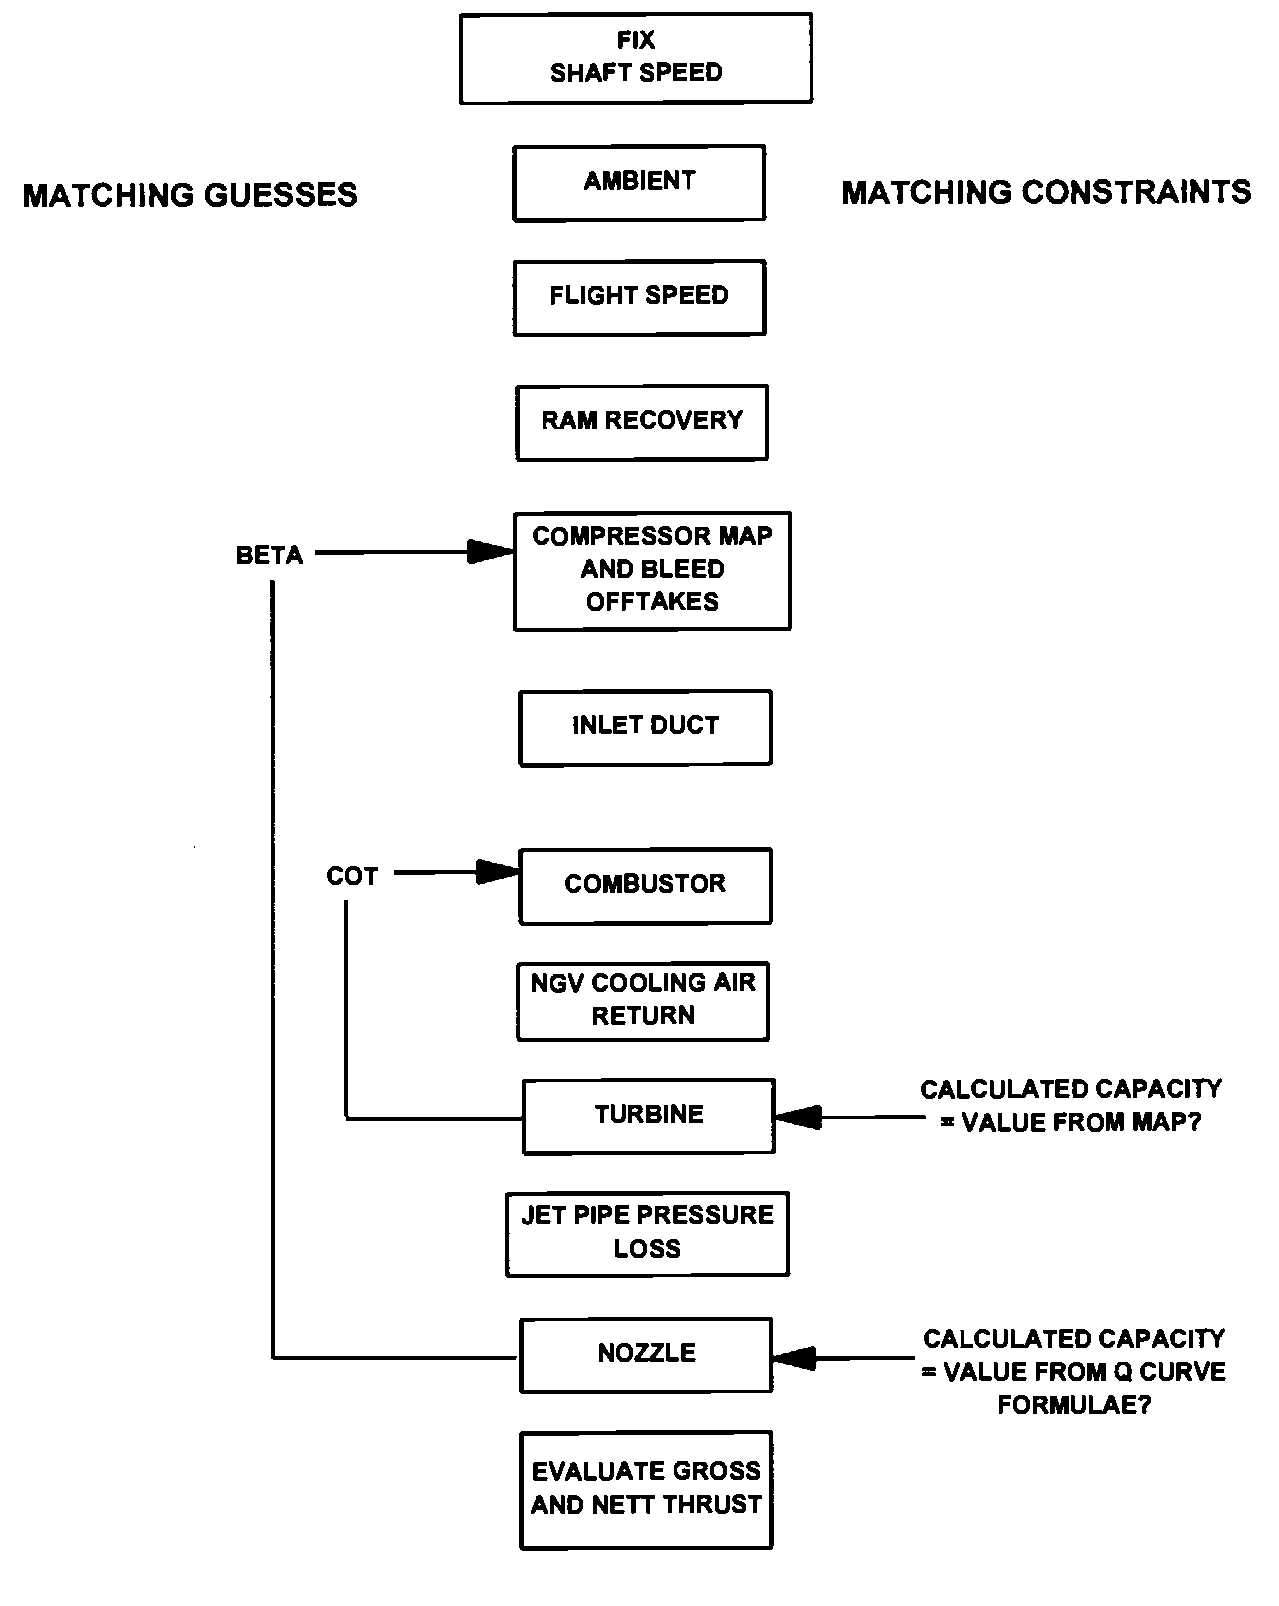
\includegraphics[width=\textwidth]{fig/transient_calculation_flowchart.png}
    \source{\cite{walsh2004gas}}
\end{figure}

\section{Architecture for computer simulation}
\section{Experimental parameter estimation}

\end{document}
